%!TEX program = xelatex
% 完整编译: xelatex -> bibtex -> xelatex*2
\documentclass[11pt,a4paper]{elegantpaper}
% \usepackage{etex}
\usepackage{xeCJK}
\usepackage{CJK}
\setCJKmainfont{STSong}
\setmainfont{Times New Roman}
\newcommand{\tm}{\fontspec{Times New Roman}}
% \newCJKfontfamily{\STSong}[AutoFakeBold={3.17}]{STSong}
\newCJKfontfamily{\heiti}[AutoFakeBold={3.17}]{SimHei}
\newCJKfontfamily{\fangsong}[AutoFakeBold = {3.17}]{FangSong_GB2312} 
\newCJKfontfamily{\huawenxingkai}[AutoFakeBold={2.17}]{STXingkai}
% \documentclass{cn}{elegantpaper}
\usepackage{fancyhdr}
\usepackage{geometry}
\usepackage{multicol}    % 正文双栏
\usepackage{abstract}    % 2栏文档,一栏摘要及关键字宏包

\usepackage{ulem}
\usepackage{amsmath}
\usepackage{graphicx}
\usepackage{caption}
\usepackage{float} %设置图片浮动位置的宏包
\usepackage{subfigure} %插入多图时用子图显示的宏包
\usepackage{amssymb}
\usepackage{listings}

\lstset{
	breaklines=true,  %代码过长则换行
	keywordstyle= \color{blue},%关键字颜色
}

\setlength{\topmargin}{-1cm}
\setlength{\oddsidemargin}{-0.9cm}  % 3.17cm - 1 inch
\setlength{\evensidemargin}{\oddsidemargin}
\setlength{\headheight}{12pt}
\setlength{\headsep}{12pt}
\setlength{\textwidth}{17.00cm}
\setlength{\textheight}{24.62cm}    % 24.62
%CDSS(VScode \LaTeX  Test)\\
\title{\Huge{\textbf{\STSong{脱丁烷塔软测量实验报告}}}\\
\LARGE{\textbf{\STSong{Project Report of Soft Sensing for Debutanizers \\ \quad }}}\\ 

\includegraphics[width=3cm]{images/1024px-Zhejiang_University_Logo.png}}
% \centering
% Zhejiang_University_Logo
\author{\normalsize 王子非,刘可佳,  李浩东  \\ \small Zifei WANG, Kejia LIU,  Haodong LI}
\institute{\normalsize 浙江大学控制科学与工程学院\\ 
\small{College of Control Science and Engineering, Zhejiang University} \\ }

\date{2022年01月13日\quad \today \\ }

\renewcommand{\headrulewidth}{0.4pt}
\usepackage{setspace}
\onehalfspacing%1.5倍行距
\addtolength{\parskip}{.4em}%段间距

\newcommand{\makeheadrule}{%
\makebox[0pt][l]{\rule[0.55\baselineskip]{\headwidth}{0.4pt}}%
\rule[0.7\baselineskip]{\headwidth}{0.4pt}}
\renewcommand{\headrule}{%
{\if@fancyplain\let\headrulewidth\plainheadrulewidth\fi
\makeheadrule}}

% 页眉页脚
\fancypagestyle{plain}{
\renewcommand{\footrulewidth}{0pt}
\fancyhf{}
\lhead{冬~学~期~课~程~报~告\quad \quad \\
\scriptsize{2022~~年~~1~~月}}
\chead{\centering{数~据~驱~动~建~模~与~应~用\\
\scriptsize{\textbf{Data Driven Modeling and Applications}}}}
\rhead{Winter Semester, Course Paper\\
\scriptsize{January, 2022}}
\cfoot{\thepage}}

% \lhead{软件复杂度与bug对软件质量的影响}
% \chead{}
% \rhead{The impact of software complexity and bugs on software quality}
% R,C,L分别代表左中右,O,E代表奇偶页
\pagestyle{fancy}
% \lhead{\rightmark}
% \rhead{\rightmark}
\chead{脱丁烷塔软测量实验报告}
\cfoot{\thepage}
\usepackage{abstract}
\newCJKfontfamily{\STSong}[AutoFakeBold={1.585}]{STSong}

\begin{document}

\newcommand{\supercite}[1]{\textsuperscript{\cite{#1}}}
\renewcommand{\thefootnote}{\Roman{footnote}}

% \begin{figure}[H]
%   \centering
%   
\includegraphics{images/1024px-Zhejiang_University_Logo.png}
% \end{figure}

\maketitle

\renewcommand{\abstractname}{\textbf{\STSong{摘\quad 要}}\\}
\begin{abstract}
\textbf{\quad\quad}摘要\footnote{摘要摘要摘要摘要摘要摘要摘要}
摘要摘要摘要摘要摘要摘要摘要摘要摘要摘要摘要摘要摘要摘要摘要摘要摘要摘要摘要
摘要摘要摘要摘要摘要摘要摘要摘要摘要摘要摘要摘要摘要摘要摘要摘要摘要摘要摘要摘要摘要
摘要摘要摘要摘要摘要摘要摘要摘要摘要摘要摘要摘要摘要摘要摘要摘要摘要
摘要摘要摘要摘要摘要摘要摘要摘要摘要摘要摘要摘要摘要摘要摘要
\\ \\ 
\textbf{\STSong{关键词}}:学习,学习,学习\\ 
\end{abstract}

\renewcommand{\abstractname}{\textbf{\STSong{Abstract}}\\}
\begin{center}
\textbf{\STSong{Abstract}}
\end{center}
% \newcommand{\abstracttextfont}{\}
\begin{quote}
  Abstract
Abstract\footnote{Abstract}
AbstractAbstract  Abstract Abstract Abstract Abstract Abstract 
Abstract Abstract Abstract Abstract Abstract .
\keywords{Key Words\\ }
\end{quote}

\begin{multicols}{2}
% \begin{twocolumn}
\section{引言}


\section{数据预处理}

\section{模型搭建}


\subsection{\lstinline{长短时记忆(LSTM)}}

\subsection{\lstinline{卷积神经网络(CNN)}}


\section{模型结果与分析}


\section{小组分工}

\section{APPENDIX: Source Code}

\subsubsection{\lstinline{filename.py}}

\begin{lstlisting}[language=Python]
print("hello world")
\end{lstlisting}


% \end{twocolumn}
\nocite{*}
\bibliography{books}
\end{multicols}
\end{document}
%%%%%%%%%%%%%%%%%%%%%%%%%%%%%%%%%%%%%%%%%%%%%%%%%%%%%%%%%%%%%%%%%%%%%%%%%%%%%%%%%%%%%%%%%%%%%%%%%%%%%%%%%%%%%%%%%%%%%%%%%%%%%%%%%%%%%%%%%%%%%%%%%%%%%%%%%%%%%%%%%%%%%%%%%%%%%%%%%%%%%%%%%%%%%%%%%%%%%%
\begin{description}
 \item[First] \hfill \\
 The first item
 \item[Second] \hfill \\
 The second item
 \item[Third] \hfill \\
 The third etc \ldots
\end{description}

\begin{equation}
(a+3b)^{n} = \sum_{k=0}^{n} C_{n}^{k} a^{n-k} (3b)^k\label{eq:binom}
\end{equation}

\begin{lstlisting}
\usepackage[UTF8,scheme=plain]{ctex}
\end{lstlisting}

\begin{enumerate}
\item 软件功能质量:
\item 软件结构质量:
\end{enumerate}

\begin{quote}
指能指挥计算机工作的程序、程序运行时所需要的数据以及与这些程序和数据有关的文档。
\end{quote}

\lstinline{}

\begin{itemize}
\item 程序是按事先设计的功能和性能要求执行的指令序列;
\item 数据是使程序能正常操纵信息的数据结构;
\item 文档是与程序开发,维护和使用有关的图文材料。
\end{itemize}

在引出本文的研究方向(软件复杂度与bug对软件质量的影响)之前,笔者首先对整体上软件的部分概念做简要陈述。

\subsection{软件的定义与内涵}
在简要浏览所给数书目后,笔者决定选择Shari Lawrence Pfleeger的著作《Software Engineering , Theory and Practice》作为本文的主要参考书目\supercite{test}。软件作为现代社会的重要部分,是一个值得研究的对象,据\href{https://en.wikipedia.org/}{维基百科(Wikipedia)}\supercite{tuantuan},软件的定义为:
\begin{quote}
\textbf{Software} is a collection of data or computer instructions that tell the computer how to work. This is in contrast to physical hardware, from which the system is built and actually performs the work.
\end{quote}
此外,课程《软件技术基础》\footnote{之后简称为:《软基》}中关于软件系统(Software)的定义是:
\begin{quote}
指能指挥计算机工作的程序、程序运行时所需要的数据以及与这些程序和数据有关的文档。
\end{quote}
定义中关于名词“程序”、“数据”、“文档”的解释为:
\begin{itemize}
\item 程序是按事先设计的功能和性能要求执行的指令序列;
\item 数据是使程序能正常操纵信息的数据结构;
\item 文档是与程序开发,维护和使用有关的图文材料。
\end{itemize}
目前关于软件的看法,往往仁者见仁,智者见智\dots

\subsection{软件与硬件的关系}
在了解过部分学者关于软件定义与内涵的看法后,笔者发现,很多学者将软件(Software)与硬件(Hardware)分开看待,正如Yale N. Patt\footnote{Yale N. Patt: Professor of Electrical and Computer Engineering,
Ernest Cockrell, Jr. Centennial Chair in Engineering, and
University Distinguished Teaching Professor,
The University of Texas at Austin}所说:
\begin{quote}
It is as if there were a big wall between the hardware (the computer and how it actually works) and the software (the programs  that  direct  the computer's  bidding), and that one should be content to remain on one side of that wall or the other.  
\end{quote}
强调软件基于硬件实现功能,却经常忽略软件与硬件之间密不可分的关联,笔者认为,只有精通软件与硬件之间的关联,才可以设计出优秀的计算机系统,Yale N. Patt在其著作《Introducion to Computing Systems (2nd Edition)》\supercite{test}中讲到:
\begin{quote}
As you approach your study and practice of computing, we urge you to take the opposite approach—that  hardware and software are names for components of two parts of a computing system that work best when they are designed by someone who took into account the capabilities and limitations of both. 
\end{quote}
真正理解计算机程序需求的硬件设计者才可以\dots

\section{软件质量}
\subsection{软件质量的定义}
软件质量可以大致分为两个方面:
\begin{enumerate}
\item 软件功能质量:基于功能需求或规格反映了其与给定设计的符合性。
\item 软件结构质量:是指软件满足需要交付的功能外的要求的优劣性,例如健壮性或可维护性。
\end{enumerate}

\subsection{软件质量的评估}
ISO9126软件质量模型(图一)是评价软件质量的国际标准,由6个特性和27个子特性组成\supercite{tuantuan}。对于大部分的软件,都可以考虑从这几个方面着手进行测评。
% \begin{figure}[htbp]
\begin{figure}[H]
  \centering
  \includegraphics[width=0.5\textwidth]{images/SQ.png}
  \caption{ISO 9126 软件质量模型} 
\end{figure}
在我国,现行的软件质量评估标准是由中华人民共和国国家质量监督检验检疫总局和中国国家标准化管理委员会共同编撰《软件质量量化评价规范\supercite{test}(Specification for the quantitative evaluation of software quality)》。

\subsection{软件质量的进一步分析}
笔者认为,软件质量可以有两个视角\dots

\begin{table*}
  \centering
  \caption{Table of students.}
  \begin{tabular*}{\hsize}{@{}@{\extracolsep{\fill}}ccc@{}}
  \hline
  Name & Age & Gender  \\ \hline
  Cat & 3  & Girl  \\ \hline
  Dog & 5 & Boy \\
  \hline
  \end{tabular*}
  \label{table:stu}
  \end{table*}

软件质量是贯穿到软件的整个生命周期中(图二),从问题定义、可行性研究、需求分析、系统设计、详细设计、编码、测试、运行与维护。一旦在某一步骤出现疏漏,就会导致几乎所有子步骤的错误(图三)。
\begin{figure}[H]
  \centering
  \includegraphics[width=0.5\textwidth]{images/LLCC.png}
  \caption{软件的生命周期} 
\end{figure}
\begin{figure}[H]
  \centering
  \includegraphics[width=0.5\textwidth]{images/358.png}
  \caption{错误的传递} 
\end{figure}
软件质量非常重要,特别是对于商业软件和系统软件(例如Microsoft Office,Microsoft Windows和Linux)\dots

\section{软件复杂度}
著名计算机研究学者Brian Kernighan\footnote{Brian Wilson Kernighan (born January 1, 1942): a Canadian computer scientist.}在其著作中指出:
\begin{quote}
Controlling complexity is the essence of computer programming.
\end{quote}
软件复杂度是软件的重要衡量指标,与软件质量的联系十分密切,下面本文将给出关于软件复杂度的论述。

\subsection{软件复杂度的定义}
软件复杂度是软件的重要属性\supercite{tuantuan}。复杂意味着\dots

\subsection{软件复杂度的分析}
\subsubsection{软件复杂度的不利影响}
软件复杂度是灵活性的敌人。软件复杂度让我们陷入不可预期的结果\dots

\subsubsection{软件复杂度的原因}
软件复杂性的产生原因十分复杂,对于软件的生命周期而言,主要有以下几点:
\begin{enumerate}
\item 需求复杂、应用要求高;
\item 开发环境复杂;
\item 软件应用框架、结构及模型复杂;
\item 软件开发过程复杂;
\item 涉及人的智力和管理复杂;
\item 项目设计与验证复杂。
\end{enumerate}

如下图所示:
\begin{figure}[H]
  \centering
  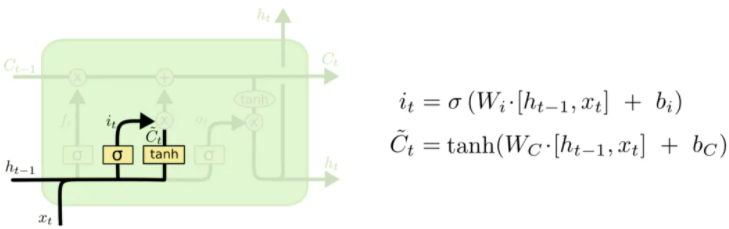
\includegraphics[width=0.5\textwidth]{images/SC.png}
  \caption{软件的复杂度} 
\end{figure}

笔者认为,现实世界本身就是复杂的。这个是本质复杂度。

\section{软件bug}
软件bug是我们所不期望遇见的,不论是软件的开发者与使用者,正如下面这段话所说:
\begin{quote}
Software will change the world, but bug will destroy it.
\end{quote}
软件bug会造成很多不同程度上的错误,其中不乏十分严重的错误,比如:
\begin{quote}
1963年,美国飞往火星的火箭爆炸,损失大约\$10 million。原因为: \lstinline{FORTRAN}循环\lstinline{DO  5  I = 1,  3}误写为\lstinline{DO  5  I = 1.3}。
\end{quote}
软件bug同样也是衡量软件质量评估的重要参考因素。下面本文将对软件bug进行论述。
\subsection{软件bug的定义}
软件bug是指计算机程序或系统中的错误\dots

\subsection{软件bug的修复}
下面,本文将从软件bug的修复成本以及软件生命周期不同阶段如何减少bug的注意事项两方面论述软件bug的修复相关内容。

\subsubsection{软件bug的修复成本}
软件bug的成本有这样一条规律:发现的越晚,修复的成本越高,比如:
\begin{quote}
软件Aspen的运行与维护:MIT 30教授为首,联合50家公司,历时五年(1976-1981)开发运行,总共耗资600万美元。
\end{quote}
在最终交付给客户的产品或者服务时发现的bug, 比引入阶段发现的bug,其影响和修复成本要高出数倍(如图五),这一点类似问题汽车的召回。
\begin{figure}[H]
  \centering
  \includegraphics[width=0.5\textwidth]{images/COST.png}
  \caption{软件bug的修复成本与发现时间的关系} 
\end{figure}
此外,在软件生命周期的不同阶段,引入的bug的数量往往是不一样的,不难理解,大约85\%的bug是在软件开发的编码时期被引入的(如图六)。
\begin{figure}[H]
  \centering
  \includegraphics[width=0.5\textwidth]{images/507.png}
  \caption{不同阶段bug的数量} 
\end{figure}
而且,不同的阶段我们能够发现的bug的数量是不一样的\dots

\subsubsection{软件bug的修复成本}
下面本文将从不同的阶段对bug的修复进行论述。
\begin{itemize}
\item 需求探索时期

这个阶段需要软件开发团队\dots

对于一个全新的产品,DesignThinking\dots

\item 软件设计时期

设计是承上启下的步骤\dots

\item 软件编码阶段

这个阶段bug引入最多\dots

\begin{enumerate}
\item Pair Programming\footnote{Pair Programming下,同一个算法、同一段代码或同一组测试、与两位程序员各自独立工作相比,往往只需花费大约一半的时间就能编写出质量更高的代码。}
\item Code Review\footnote{Code Review:代码评审也称代码复查,是指通过阅读代码来检查源代码与编码标准的符合性以及代码质量的活动。}
\item  Code Inspect\footnote{Code Inspect:IDE的静态分析。}
\item SCS(Static Code Scan)\footnote{Static Code Scan:在软件工程中,程序员在写好源代码后,无需经过编译器编译,而直接使用一些扫描工具对其进行扫描,找出代码当中存在的一些安全漏洞的解决方案。}
\item Unittest\footnote{Unittest是一种完整的测试结构,支持自动化测试的执行,对测试用例集进行组织,并且提供了丰富的断言方法,最后生成测试报告。}
\item TDD(Test-Driven Development)\footnote{TDD是一种软件工程实践,要求在应该验证的代码之前编写单元测试。}(如图七)
\end{enumerate}

\begin{figure}[H]
  \centering
  \includegraphics[width=0.5\textwidth]{images/TDD.png}
  \caption{TDD Cycle} 
\end{figure}

\item 软件的运维阶段

传统软件发布是一个安装包\dots
\begin{enumerate}
\item 运行环境的监控
\item 应用程序的黑盒监控
\item log的信息
\end{enumerate}
其中log里面的warning 和error一定要去留意\dots
\end{itemize}

\section{结语}
结语。
